\documentclass{mproj}
\usepackage{graphicx}

\usepackage{url}
\usepackage{fancyvrb}
\usepackage[final]{pdfpages}
\usepackage{times}
\usepackage{gensymb}
\usepackage{colortbl}
\usepackage{booktabs}
\usepackage{amsmath}
\usepackage[linesnumbered,ruled]{algorithm2e}
\usepackage{tikz}
\def\checkmark{\tikz\fill[scale=0.4](0,.35) -- (.25,0) -- (1,.7) -- (.25,.15) -- cycle;} 

% for alternative page numbering use the following package
% and see documentation for commands
%\usepackage{fancyheadings}


% other potentially useful packages
%\uspackage{amssymb,amsmath}
%\usepackage{url}
%\usepackage{fancyvrb}
%\usepackage[final]{pdfpages}

\begin{document}
%%%%%%%%%%%%%%%%%%%%%%%%%%%%%%%%%%%%%%%%%%%%%%%%%%%%%%%%%%%%%%%%%%%
\title{Title of project placed here}
\author{Michael Georgiev}
\date{Date of submission placed here}
\maketitle
%%%%%%%%%%%%%%%%%%%%%%%%%%%%%%%%%%%%%%%%%%%%%%%%%%%%%%%%%%%%%%%%%%%

%%%%%%%%%%%%%%%%%%%%%%%%%%%%%%%%%%%%%%%%%%%%%%%%%%%%%%%%%%%%%%%%%%%
\begin{abstract}
abstract goes here
\end{abstract}
%%%%%%%%%%%%%%%%%%%%%%%%%%%%%%%%%%%%%%%%%%%%%%%%%%%%%%%%%%%%%%%%%%%

%%%%%%%%%%%%%%%%%%%%%%%%%%%%%%%%%%%%%%%%%%%%%%%%%%%%%%%%%%%%%%%%%%%
\educationalconsent

%%%%%%%%%%%%%%%%%%%%%%%%%%%%%%%%%%%%%%%%%%%%%%%%%%%%%%%%%%%%%%%%%%%

\newpage
%%%%%%%%%%%%%%%%%%%%%%%%%%%%%%%%%%%%%%%%%%%%%%%%%%%%%%%%%%%%%%%%%%%
\section*{Acknowledgements}

Yo! If you are reading this... I love you $<3$ You will be my acknowledgement.

%%%%%%%%%%%%%%%%%%%%%%%%%%%%%%%%%%%%%%%%%%%%%%%%%%%%%%%%%%%%%%%%%%%
\tableofcontents
%%%%%%%%%%%%%%%%%%%%%%%%%%%%%%%%%%%%%%%%%%%%%%%%%%%%%%%%%%%%%%%%%%%

%%%%%%%%%%%%%%%%%%%%%%%%%%%%%%%%%%%%%%%%%%%%%%%%%%%%%%%%%%%%%%%%%%%
\chapter{Introduction}\label{intro}

\section{Sentence}

I completed a program which allowed a turtlebot to autonomously map an environment using SLAM as well as create an inventory of items found in the environment.


\section{Importance/Context/Motivation}

Mobile robots are becoming more and more affordable and accessible which has allowed developers to take advantage of their applications in many different ways. 

SLAM has it's application in rescue robots which
http://www.aaai.org/Pressroom/Releases/release-02-0910.php
these robots required realtime control and utilised only video streams to identify and rescue people.

This compares to this which utilises rugged mobile robots to create SLAM maps of mine shafts with minimal supersvision. This can then be applied to areas which are too unsafe/ small for humans to access.
https://miningrox.informatik.tu-freiberg.de/en/

More affordable Drones can also be used to increasingly accurate create maps of property as well

Object detection can be used to detect humans via heat sensors etc. Aswell as identifying bombs etc.



\section{Objectives/Problem statement}

While the Turtlebot has been increasingly used by developers and researchers to create robotic software much of this development has been in focused and isolated components and not combined into useful applications. Similarly much work has primarily been developed using simulated environments and not tested using the Turtlebot or cameras.

The objective of this project is to build a prototypical system which combines pre-built SLAM software with frontier exploration and implements a bespoke object detection and recognition service on the Turtlebot. When placed in an unknown room the Turtlebot will autonomously create a 3D map of the environment while creating an inventory of classified and localised objects in the map.

\section{System Overview} 

\subsection{System Diagram} 
\subsection{How I achieved it}

\section{Outline of the dissertation} 




%%%%%%%%%%%%%%%%%%%%%%%%%%%%%%%%%%%%%%%%%%%%%%%%%%%%%%%%%%%%%%%%%%%
\chapter{Background}\label{survey}

This chapter provides research into the hardware and software required to run the Turtlebot and perform autonomous SLAM mapping.
It will consider the processes of object detection and recognition by first considered them in the context of natural visual systems and then in application in software.

\section{Mobile Robots}


Mobile robots are robots that are not fixed to one location and are capable of moving around their environments. Movement is achieved generally through legs, wheels or tracks but aerial and nautical robots can use propellors. The robot can be controlled through manual-tele operation involving a human driver, line-following which follow visual cues such as painted lines to navigate or autonomously. These robots have many applications in areas such as the military, agriculture, rescue, transport and domestic use and include Unmanned Aerial Vehicles (UAVs or more commonly known as drones)and self-driving cars.

\subsection{Turtlebot 2}

The Turtlebot 2 is a part of a series of low cost, open-source mobile robots first developed at Willow Garage by Melonee Wise and Tully Foote in 2010. These robots are intended for educational and research purposes and provide an 'low-barrier-of-entry' platform for development while suitable hardware for SLAM and navigation\cite{turtlebot}. The construction of the robot is very flexible featuring a modular support structure that encourages adding additional hardware but the core of the Turtlebot consists of a Kobuki base, a computer running ROS and some form of camera particularly RGB-D or stereo cameras such as the Xbox Kinect or Zed Camera.

\begin{figure}[h]
  \caption{The Turtlebot used for the project. Featuring a Zed Camera and Lenovo Ideapad Y700.}
  \centering
  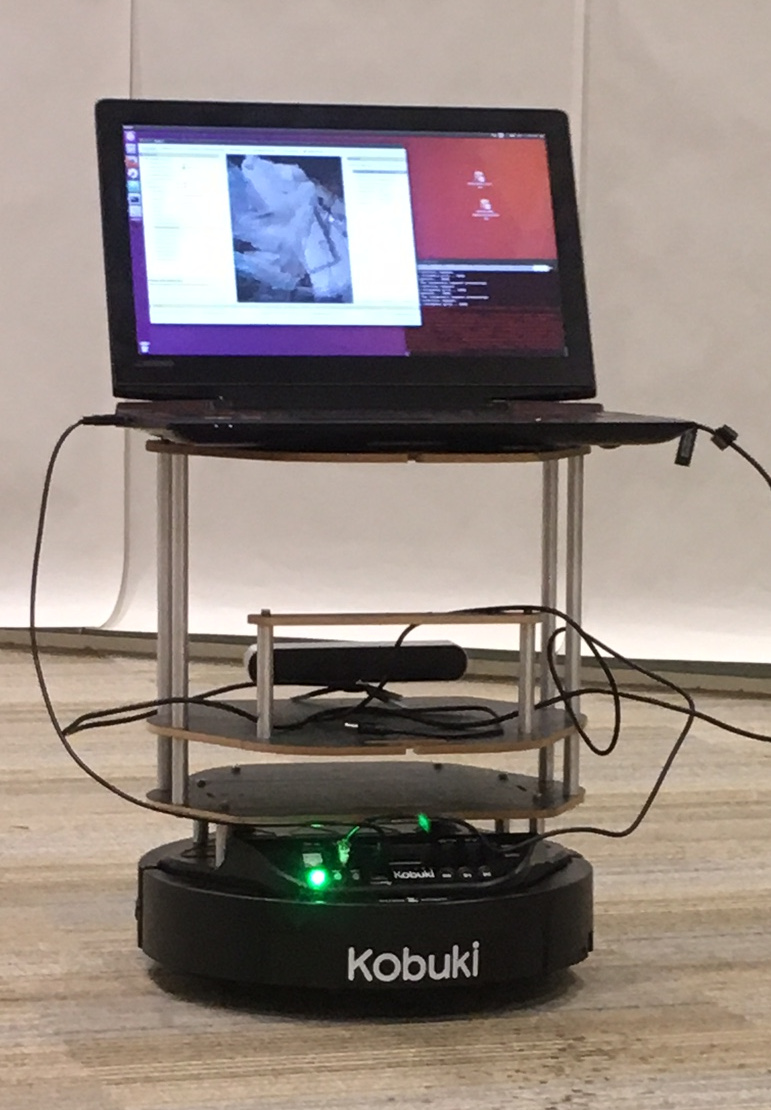
\includegraphics[width=0.5\textwidth]{images/turtlebot.JPG}
  \label{fig:Turtlebot}
\end{figure}
 
The Kobuki base contains sensors and actuators as well as a power supply and vehicular functions. This provides a centralised unit of hardware that can be accessed via the Robot Operating System (ROS). This means that hardware processes are sufficiently abstracted as to be approachable for software developers and other high-level users without an engineering or robotics background. The base has cliff, wheel drop and bumper sensors as well as a gyroscope and highly accurate odometry. 

As it requires a computer running ROS to communicate with, a laptop can simply be attached to the top of the base connected by a USB cable. However, in some cases it may be more convienent to attach a small netbook or Raspberry Pi to the base and then use a seperate computer to remotely communicate with the host machine. The Turtlebot has many bespoke packages for use within ROS, these include standard applications such as teleoperation or navigation and more specialized packages such as frontier exploration. 


\subsection{Cameras}
For nearly all use cases, the Turtlebot requires the use of a camera. While this can be something as simple as a webcam a greater number of applications can be created for it with some form of depth or range measurement received from RGB-D and stereo cameras. Both the discussed cameras are commonly used in ROS and for the Turtlebot.

The Kinect is a very affordable RGB-D camera developed for use on machines running Microsoft Windows though open-source drivers exist for other operating systems. The Kinect is an active camera which utilises a time-of-flight sensor to estimate the distance of points in the field of view. The Zed Camera is a stereo camera with a very user-friendly SDK and wide driver support. 

\begin{table}[ht]
\caption{Comparison of the Zed Camera and Xbox Kinect v2}
\centering 
\begin{tabular}{c | c | c  }
\hline
 \rowcolor{gray!50}Feature     & Kinect         & Zed Camera \\
 \hline
 Resolution  & 1080p at 30fps & 1080p at 30fps \\
 Depth range & 0.5 - 8m       & 0.5 - 20m \\
 FOV         & 70\degree horz. and 60\degree vert. & 110\degree \\
 Power       & 12V Adapter	  & 5V USB \\			  
\bottomrule
\hline
\end{tabular}
\label{table:camera comparison}
\end{table}

\section{Robot Operating System (ROS)}

ROS is a meta-operating system which provides a collection of tools and conventions to aid the writing of robot software. This includes an abstraction of hardware and communications as well as many tools for tasks such as message passing and package management.

ROS features open-source licenses and a large growing collection of packages which contribute to a vibrant ecosystem of developers and researchers working on applications. Some of these packages provide frameworks and algorithms for areas such SLAM and kinematics as well as useful visual and modelling tools. These include:

\begin{itemize}
  \item \textbf{RViz} - a visualisation tool which provides 3D visualisations of sensor data and robot states, such as cameras, lasers and joint states.
 \item \textbf{Gazebo} - a modelling tool which provides a simulated environment to build and test applications in ROS complete with robot sensors and accurate physics.
\end{itemize}


The software engineering principles of loose coupling and abstraction are encouraged throughout design which simplifies software integration and reuse as well as meaning that ROS is generally independent of hardware specifics. ROS features standard implementations in popular programming languages such as Python and C++ which has further increased the community of users.

\subsection{How does ROS work?}

ROS consists of some key components within the communications infrastructure.
\begin{itemize}
  \item \textbf{Nodes} are modular processes performing computation which can communicate with each other using topics or services. A system may consist of many nodes which perform many different tasks.
  \item \textbf{Topics} are named buses which provide a clear message passing interface between nodes. This is achieved through an anonymous publish/subscribe mechanism that allows many-to-many transport.
  \item \textbf{Messages} are a data structure which are published by nodes to topics. They support strongly typed fields such as primitives or arrays and are either predefined or user-defined.
  \item The ROS core or \textbf{Master} provides a centralized node which locates and negotiates communications between nodes as well providing naming and registration services.
  \item \textbf{Services} forgo the many-to-many paradigm and provide a request/reply interaction via servers and clients.
\end{itemize}

\begin{figure}[h]
  \caption{Illustration of general ROS communication concepts}
  \centering
  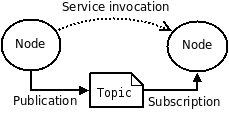
\includegraphics[width=0.5\textwidth]{images/ROS_basic_concepts.png}
  \label{fig:ROS diagram}
\end{figure}

* DIAGRAM OF DESCRIBED SYSTEM

For example a simple robot vehicle system can consist of three nodes. The first node controls the robot's ultrasonic range finder and is publishing a stream of range messages taken from the sensor along the \texttt{sensor/sonar} topic.

The second node controls the robot's movement hardware and is publishing the robot's orientation on the \texttt{geometry\char`_msgs/pose} topic. It also contains an actionlib server which responses to requests to change the robot's positioning. 

The third node controls the robot's movement and is subscribed to the \texttt{sensor/sonar} topic and contains a client of the actionlib server. While processing the range messages, if the range indicated is very small the node can use the actionlib service to request an adjustment in the orientation of the robot thus meaning the robot will avoid collisions. 



\section{SLAM (Simultaneous Localisation and Mapping)}

SLAM is the problem of simultaneously localising (finding the pose and orientation) of a camera within it's surroundings at the same time as mapping the structure of the environment. This requires a robot or camera with the ability to produce odometry readings as well as a camera with a range measurement device.

SLAM forms the basis of navigation in most mobile robots, meaning unknown environments can be explored and mapped without the need for technology such as GPS which is not precise. It has applications in a range of manned and autonomous robots. This includes UAVs, underwater robots and domestic robots such automatic lawnmowers. SLAM is also a key component in the development of self-driving cars These cars are driven along routes while performing SLAM capturing location, feature and obstacle data. Once the map is completed it is processed and the cars are driven autonomously along these routes updating the map as necessary.


\begin{figure}[h]
  \caption{Illustration of the SLAM problem.}
  \centering
  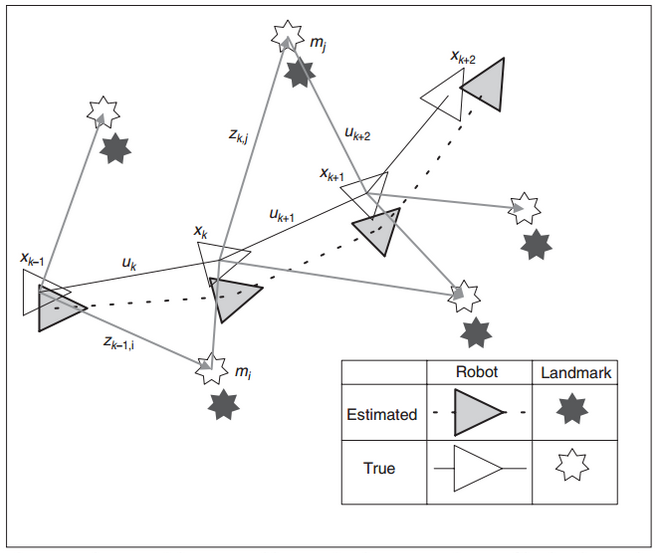
\includegraphics[width=0.5\textwidth]{images/slam_problem.png}
  \label{fig:SLAM Problem}
\end{figure}
https://blog.acolyer.org/2015/11/05/simultaneous-localization-and-mapping-part-i-history-of-the-slam-problem/

This is considered to be a solved problem in Computer Science and their are many different approaches for finding a solution \cite{Hugh2006}. But at a high level SLAM is solved by using the environment to update the pose of the robot. Using odometry as the sole measurement of localisation has an element of uncertainity due to extraneous factors such as wheels slipping on different environments meaning that a stated distance given by an odometry reading may be over or under estimated. 

Therefore laser scans or other forms of depth readings are used to correct the robot's position by extracting features from the surrounding environment. These are called landmarks and can be extracted by various methods such as Random Sampling Consensus (RANSAC) and provide a growing map of the enviroment. Recognising previously visited landmarks is process known as loop closure detection where matches are found between new observations  and regions of the map determined by the uncertainty associated  with the robot’s position\cite{labbe13appearance}.

Most SLAM solutions are probalistic and for example, can use a Kalman to track the uncertanity of the robot within the map using erroneous range observations and robot controls such as odometry over time. Formally:

\[ \textit{P}\left(x, m | z_{1:t}, u_{1:t}\right) \]

Where:

Given:

Robot controls $ u_{1:t} = \lbrace u_{1}, u_{2}, u_{3} ... u_{t} \rbrace $

Observations $ z_{1:t} = \lbrace z_{1}, z_{2}, z_{3} ... z_{t} \rbrace $

Wanted:

Map of the Environment $ m $

Path of the robot $ x_{0:t} = \lbrace x_{1}, x_{2}, x_{3} ... x_{t} \rbrace $

(Starts at 0 to fix a coordinate frame)


SLAM was considered an especially difficult problem to solve \cite{Hugh1988} because these variables cannot be fully decoupled as can be observed in Figure []???. For example a map is required for localising landmarks  which requires pose estimates.

\begin{figure}[h]
  \caption{Graph illustrating the dependencies between SLAM variables.}
  \centering
  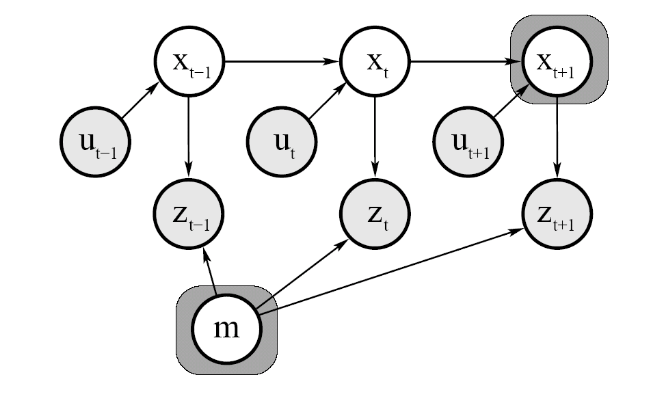
\includegraphics[width=0.5\textwidth]{images/slam_graph.png}
  \label{fig:SLAM Graph}
\end{figure}


\subsection{RTABMap}

ROS features many different applications of SLAM including a popular wrapper for OpenSlam's Gmapping which produces a 2D occupational grid map.\cite{gmapping} Another approach is RTABmap (Real-Time Appearance-Based Mapping) which produces a 3D point cloud map as well as 2D occupancy grid map. It is a RGB-D Graph-Based approach based on an incremental appearance-based loop closure detector. 

\begin{figure}[h]
  \caption{Graph  representation  of  locations.  Vertical  arrows  are  loop  closure
links and horizontal arrows are neighbour links. Dotted links show not detected
loop closures. Black locations are those in LTM, white ones are in WM and
gray ones are in STM. Node 455 is the current acquired location}
  \centering
  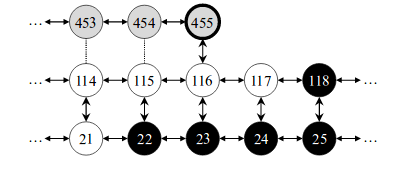
\includegraphics[width=0.5\textwidth]{images/graph.png}
  \label{fig:RTABMap Graph diagram}
\end{figure}

In most probablistic SLAM approaches loop closure detection compares newly found landmarks to previously visited landmarks. This takes an exponential amount of time as the time required to process new landmarks increases with the number of visited landmarks found on the map. A delay is introduced if this process is greater than the time it takes to find a new landmark thus deteriorating the accuracy of the map produced.
 
\begin{figure}[h]
  \caption{RTAB-Map memory management model.}
  \centering
  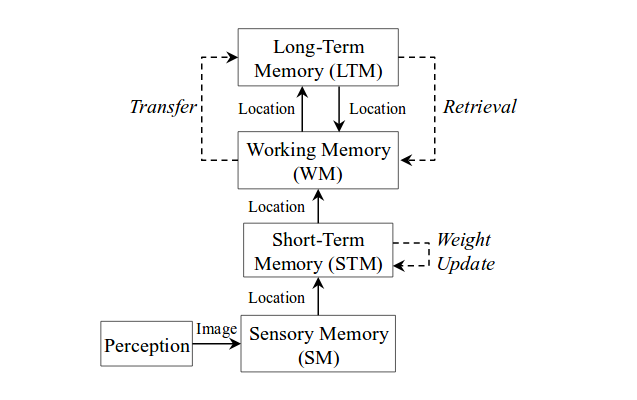
\includegraphics[width=0.5\textwidth]{images/memory.png}
  \label{fig:RTABMap Memory diagram}
\end{figure}

RTAB-Map uses an efficient memory management technique to minimise this problem by keeping the most frequent and recently observed landmarks in the robot's Working Memory (WM) and transfers the others into a Long-Term Memory(LTM). \cite{labbe13appearance} Locations in LTM are not used for loop closure detection and thus a weighting system using a graph of landmarks is used. When  landmarks need to be transfered from  WM to LTM the landmark with the lowest weight is selected. 


\section{Object Detection and Classification}

\subsection{Introduction}
Object detection is the task of finding the potential real-world objects within images or videos while classification involves giving these objects the correct label. Alongside robotics, such technology has applications in areas such as surveillance, medical image analysis and human computer interaction. Modelling a intelligent agent that interprets objects in scenes can be modelled on natural visual systems as many organism's vision systems have much less resolution, sensitivity and field of vision than a modern camera yet are able to perform incredibly complex tasks successfully. 

It is useful to think of object detection software in terms of an intelligent agent which is an autonomous entity that gathers and observers information through sensors and acts upon an environment using actuators to direct its activity to achieve goals.\cite{Norvig2003} Why???


\subsection{Detection in the Natural World}

For most visual systems while everything is seen for the first time our senses do not keep telling us things we already know, this is because between scenes, most important environmental information stays constant. This process is a form of sensory adaption where perception is temporarily changed when exposed to new stimuli in an attempt to normalise visual experience.\cite{Webster2015} This happens at a retinal and neural level, where information provided by past experience have a greater say on how a scene has been interpreted than immediate information provided by external organs. 

For example an ellipse projected into a human retina can be interpreted as a circle due to our experiences with perspective. 
%\cite{The eye the brain the computer p208}

Many species exhibit a form of pattern or feature detection to trigger neural responses to visual changes. In contrast to humans which detect generic images features such as shapes, many lower organisms utilise goal-based feature detection. This is useful to the field of computer science because it allows us to model intelligence agents on such processes, which are typically simple and linear in that there is only one way of achieving the goal and that task assumes the agents complete engagement.

For example arthopods such as honey bees readily distinguish features such as flowers in the environment that pertain to the goal of gathering food. Similarly a frog's eye is stimulated when a black disc moves in an arc rapidly within the receptor field indicating that a flying insect is near and triggers the frogs feeding response \cite{} thus satisfying the goal of feeding.

\subsection{Extracting Features}

What determines if an area of a scene is worth triggering neural activity is different for different species. In image processing software attempts are made to find features which are unique, that can be easily tracked and can be easily compared. These features can be used for many different types of processing such as calculating a histogram of oriented gradients (HOG) which can then used for object classifiers.

\subsubsection{FAST Feature Detection}

There are many software applications of feature detection, this includes SIFT (Scale-Invariant Feature Transform) which performs extremely well in most contexts\cite{Mikolajczyk}. However for applications in real-time image processing such as SLAM and Augmented Reality it is often not fast enough. FAST (Features from Accelerated Segment Test) \cite{rosten_2006_machine}\cite{rosten_2005_annotations} avoids the costly difference of Gaussians (DoG) method found in SIFT and is subsequently much faster.

Using an appropriate threshold $T$ which is usually 12, the algorithm selects a pixel $P$ which is the centre of a circle with a circumference of 16 pixels, $n$ and the pixel's $P$ intensity is $I_{p}$. The pixel $P$ is determined to be a corner if $n$ are all brighter than $I_{p} + t$ or are all darker than $I_{p} - t$. 

\begin{figure}[h]
  \caption{Illustration of the FAST}
  \centering
  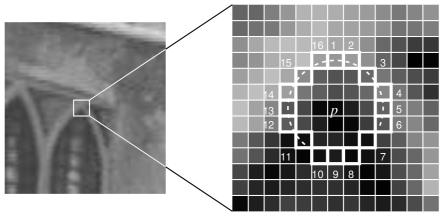
\includegraphics[width=0.5\textwidth]{images/fast_speedtest.jpg}
  \label{fig:FAST diagram}
\end{figure}

If a threshold $T$ of 12 or greater is used a high speed test is performed to reject a large number of non-corner points which involves examining the pixels at 1, 9, 5, 13. If either pixel 1 or 9 are brighter or darker than $T$ then 5 and 13 are checked. Therefore, if three of these pixels are either all darker than the threshold or all brighter then $P$ is determined to be a corner. 

\subsection{Object Classification with Deep Learning}

Determining what an object is is from within an image generally requires a form of  classifier which utilises a training set of identified images and a validation set. One such approach is Deep Learning which is based on the way the human brain processes information and learns. Deep Learning is a form of machine learning that involves feeding data through neural networks composed of many layers. This allows data to be processed in a hierarchical way where each layer recognizes higher or more abstract features than the previous layer.

\begin{figure}[h]
  \caption{Need to add******}
  \centering
  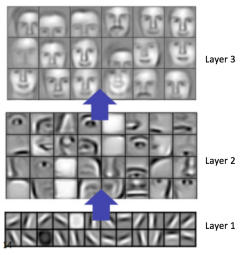
\includegraphics[width=0.5\textwidth]{images/layers.png}
  \label{fig:Deep Net Layers diagram}
\end{figure}


\subsubsection{Convolutional Neural Networks (CNN)}
  
Convolutional Neural Networks (CNN) are a type of deep neural network which since 2012\cite{} has been  increasingly popular and suited for object recognition and classification in images. This is namely because:

\begin{itemize}
\item it is rugged to distortions such as different lighting and  occlusion
\item training can be spread across several GPU's resulting in very deep networks
\item it features fewer parameters than standard neural networks meaning training time is substantially reduced
\end{itemize}

A CNN uses many identical copies of the same neuron, meaning the network can have a large amount of neurons thus expressing computationally large models while keeping the parameters the neurons have to learn very small. \cite{NIPS2012_4824}
  
An approach called \textit{symmetry} is used to look for properties in the data where at each segment of data we care about the same properties at the same time. Therefore a group of neurons, $A$ can be introduced to a neural network that computes certain features such as the presence of an edge and then the output of this layer is fed into a fully-connected layer, $F$. ****Not convincing
  
\begin{figure}[h]
  \caption{The convolutional layer is represented by the group of neurons $A$.}
  \centering
  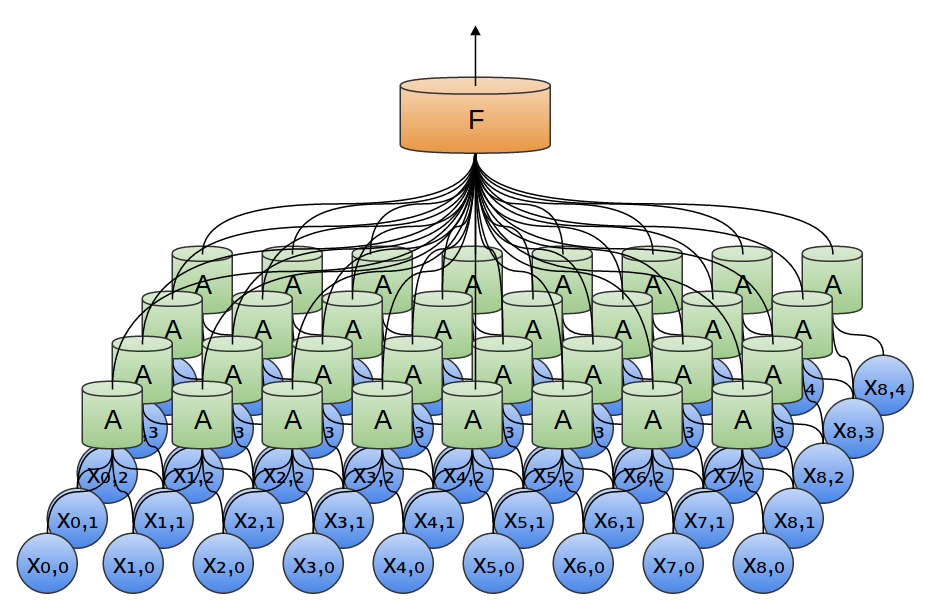
\includegraphics[width=0.5\textwidth]{images/conv.png}
  \label{fig:Basic CNN diagram}
\end{figure}

These convolutional layers are composable, meaning you can feed the output into the input of another layer detecting more abstract features. A max-pooling layer is often used which takes the maximum features over segments of a previous layer, this allows further convultional layers to work on larger sections of the data, this works because it is not wholly useful to know the exact pixel position of an edge but it is enough to know it's location within a few pixels.
 
\begin{figure}[h]
  \caption{Featuring a max-pooling layer}
  \centering
  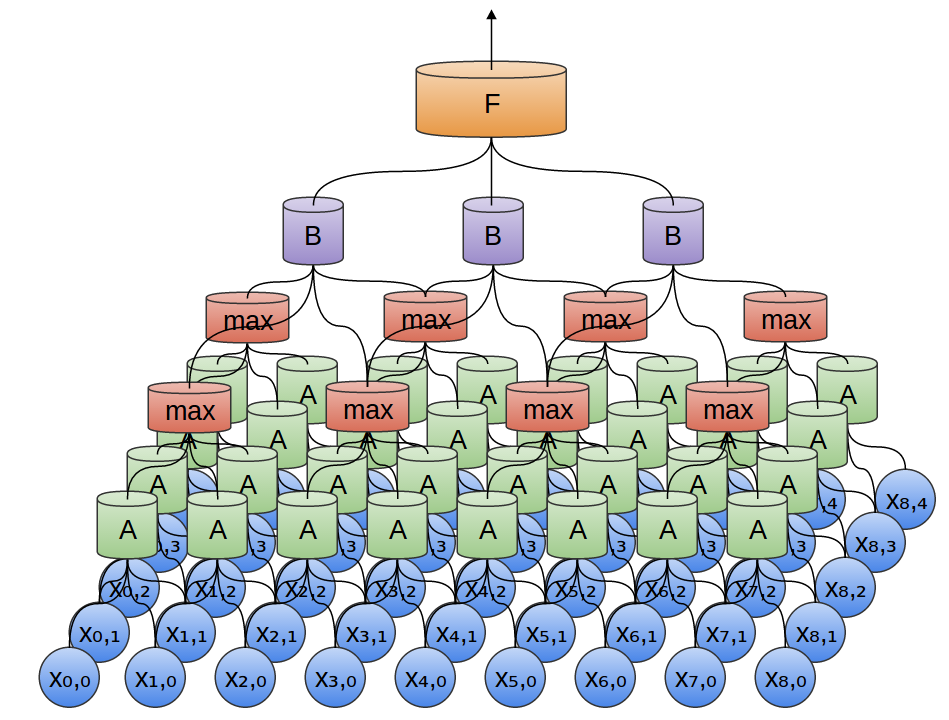
\includegraphics[width=0.5\textwidth]{images/conv_max.png}
  \label{fig:Basic CNN with Max-pooling diagram}
\end{figure}

At every convolution an element-wise operation called Rectified Linear Unit (RelU)is performed that replaces negative pixel values with zeros. This introduces non-linearity into the network because most real world data is linear.

http://colah.github.io/posts/2014-07-Conv-Nets-Modular/

\subsubsection{MobileNet with TensorFlow}
TensorFlow is an open source software library produced by Google Brain for machine learning. It is frequently used due to the fact that it discovers and uses GPUs and multiple cores by default allocating 100\% of GPU RAM for each process, this results in a very high performance. In TensorFlow, computations are represented as a graph, nodes are representations of operations and edges are multi-dimensional arrays called tensors (represented as numpy in Python). This graph occurs within a session and is executed on the CPU or GPU. 
  
MobileNet is a is a deep convolutional neural network for image recognition found in TensorFlow\cite{HowardZCKWWAA17}. The model has been trained on the 2012 ImageNet dataset and is highly optimized for efficiency and size at the expense of accuracy. However the error rate of not providing a correct classification within the top five results is only 10.5\% which for most applications is adequate. Like most pre-trained models it can be retrained to solve specific problems. This network has been used for real-time classifications on memory scarce devices and is particularly applicable to robotics.
  
  \subsubsection{Google Vision API}
  
The Google Vision API is a cloud implementation of a deep convolutional neural networks trained from Google images and implemented with TensorFlow. As part of the Google Cloud platform users can make RESTful API calls from their language of choice querying images to be classified. The service provides label detection and facial detection amongst other features such as SafeSearch which filters images based on their obscene content\cite{googlevision}.

\subsection{Regions with Convolutional Neural Networks (R-CNN)}

Detection systems utilise classifiers to evaluate potential objects. Yet there is no standard way of localising objects within an image which is often in robotics for example to estimate the distance of such object. One such approach is called Regions with Convolutional Neural Networks (R-CNN) and is considerable more efficient than previous approaches and at the time of it's release, R-CNN had the best detection performance on the PASCAL VOC 2012 image dataset. In the paper "Rich Feature Hierarchies For Accurate Object Detection and Semantic Segmentation"\cite{Girshick2014} the authors suggest a method which involves taking an image and identifying objects using bounding boxes and then performing a classification on these areas to create a label for each object. 

\begin{figure}[h]
  \caption{Illustration of the stages found in R-CNN}
  \centering
  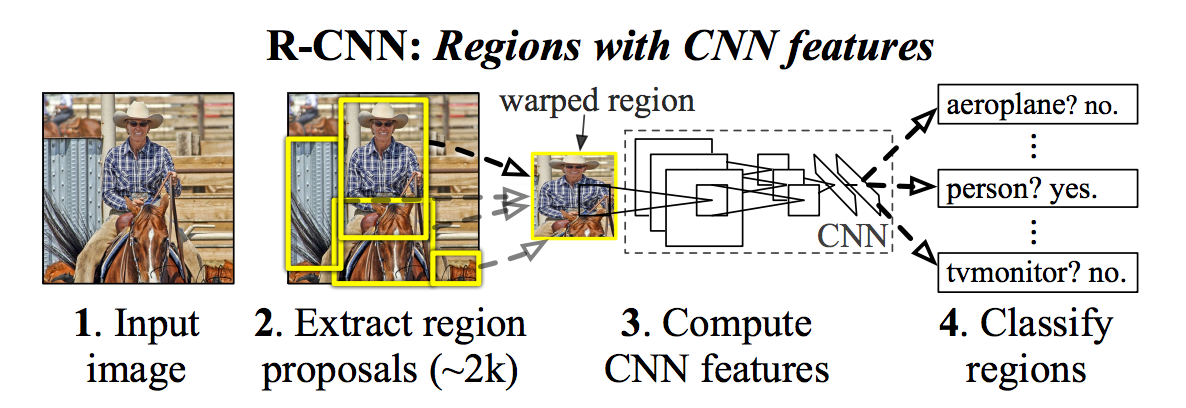
\includegraphics[width=1.0\textwidth]{images/RCNN.png}
  \label{fig:RCNN Diagram}
\end{figure}

Roughly two thousand bounding boxes, or region proposals are created using the process of Selective Search which performs a segmentation algorithm that groups regions together by color, intensity or texture.\cite{Sande2013} This is in contrast to using an exhaustive sliding window approach found in Deformable Parts Models.\cite{voc-release4} Each selected region is warped to a 227 x 227 square RGB image and fed through a CNN which computes features. The final stage involves running a Support Vector Machine (SVM) on the feature vector of each region to classify and score the object within the region (if any). Greedy non-maximum suppression is used to merge the regions which share the same object resulting in accurate bounding boxes for each object. 


\section{Summary and Discussion}
\subsection{What currently exists for completing the objectives}
\subsection{What are the my knowledge gaps, What do I have to do to fill the gaps}
\subsection{What methods are not appropriate}

%%%%%%%%%%%%%%%%%%%%%%%%%%%%%%%%%%%%%%%%%%%%%%%%%%%%%%%%%%%%%%%%%%%
\chapter{System Design}

This chapter first examines and prioritises the different requirements of the project. Then considering these requirements, this chapter will identify different approaches to fufil the project objective. These approaches will be discussed in context of their feasibility and potential successfulness. Finally a high-level description of the system design will be provided. 

\section{Requirements}
 
The problem statement/objective of this project is broad enough that it can be interpreted in many different ways. Therefore at the beginning stage of the project key system requirements were developed which help create an overaching system design and well as create a focused implementation stage. These are divided into functional and non-functional requirements. A functional requirement specifies a behaviour of the system, while a non-functional requirement describes a constraint of how the system must be developed. The defined requirements are prioritised in a MoSCoW table which states whether the requirement is Must have, Should have, Could have or Won’t have

\subsection{Functional Requirements}
\begin{itemize}
\item Autonomously explore an unknown environment
\item Perform SLAM mapping
\item Perform autonomous SLAM mapping of an unknown environment
\item Locate areas of a map which may contain potential objects
\item Locate and map predefined objects within the environment
\item Locate, classify and map undefined objects within the environment
\item Display discovered objects in the map
\item Display a 3D map of the environment
\item Visually distinguish between predefined and undefined objects
\item Allow localisation of previously mapped environment
\item Display discovered objects from within a GUI
\item Perform calibration for different environments
\item Actively create a 3D point cloud of detected objects
\item Create a database of features for detected objects
\item Navigate to object within localised map 
\item Save a map and detected object locations
\item Create a contour map of object locations
\end{itemize}
 
\subsection{Non-Functional Requirements}
\begin{itemize}
\item Turtlebot maps a sufficiently large room with in real-time
\item Object detection and recognition runs concurrently to mapping
\item Turtlebot maps different room environments (e.g. different floor and wall types)
\item Produce sufficiently accurate object classification
\end{itemize}

\subsubsection{Platform Requirements}
\begin{itemize}
\item Use ROS with Ubuntu v16.04
\item Use a Kinect v2 RGB-D camera
\item Use a ZED stereo camera
\item Use a Intel Realsense ZR300 camera
\item Application be able to be simulated in Gazebo
\end{itemize}

 \subsection{MOSCOW TABLE}

\begin{tabular}{*5l}    \toprule
\emph{Prority} & \emph{Requirement} & \emph{Version} \\\midrule
\rowcolor{green!50} Must have & Perform SLAM mapping & 1\\
\rowcolor{green!50} & Autonomously explore an unknown environment & Functional\\
\rowcolor{green!50} & Perform autonomous SLAM mapping of an unknown environment & Functional\\
\rowcolor{green!50} & Locate areas of a map which may contain potential objects & Functional\\
\rowcolor{green!50} & Locate and map predefined objects within the environment & Functional\\
\rowcolor{green!50} & Display a 3D map of the environment & Functional\\
\rowcolor{green!50} & Perform SLAM mapping & Functional\\
\rowcolor{yellow!50} Should have & Locate, classify and map undefined objects within the environment & Functional\\
\rowcolor{yellow!50} & Visually distinguish between predefined and undefined objects & Functional\\
\rowcolor{yellow!50} & Display discovered objects from within a GUI & Functional\\
\rowcolor{yellow!50} & Allow localisation of previously mapped environment  & Functional\\
\rowcolor{orange!50} Could have & Perform calibration for different environments  & Functional\\
\rowcolor{orange!50} & Navigate to object within localised map  & Functional\\
\rowcolor{orange!50} & Save a map and detected object locations  & Functional\\
\rowcolor{red!50} Would like & Create a contour map of object locations & Functional\\
\rowcolor{red!50} & Create a database of features for detected objects & Functional\\
\rowcolor{red!50} & Actively create a 3D point cloud of detected objects & Functional\\

\bottomrule
 \hline
\end{tabular}


\section{Design Approach}

The project will consist of four main processes, SLAM mapping, exploration, object detection and recognition and visualisation. It will utilise a pre-built SLAM package for mapping and which will be adapted to work with the Turtlebot and the desired cameras. A pre-built frontier exploration package will also be used but will have to be adapted to work with the Turtlebot and the object detection processes. Object detection and recognition will be created from scratch for use with a map building robot and the desired cameras. Finally visualisation will be handled primarily by RViz. The stated design approach is a composite, having been informed by many different alternative approaches

\subsection{Alternative Approaches}

\begin{enumerate}
\item Utilise prebuilt software for all components of the system. The project would stitch them together while providing a facade for user interaction. - This approach would require using a general purpose object recognition system which would not easily provide the localisation of objects in a 3D map without editing the source code. This would task would involve decomposing very large and complex systems which is unnessessary. Similarly, stitching together components means the project will be highly coupled to external software which may affect futureproofing and futher reuse.
\item Create a bespoke object detection package which by default does not need a map, but has functionality to locate objects within a map. This would also require incorporating external packages for SLAM etc. into the project. - This approach would produce a highly reusable generic object detection service that could be used with just a RGB-D or Stereo camera. However, this is not required to achieve the project objectives and would require substantial research and time invested into developing a process of maintaining  persistance when tracking objects in a 2D image.
\item Create a package from scratch which would solve simple SLAM while providing exploration and object detection. - This approach  would require a considerable amount of time and an advanced background in mathematics.
\end{enumerate}


\section{System Architecture}

Due to there being many different ways to implement the project at a low-level either by choice of technology or algorithms etc. a high-level system architecture diagram will be discussed. The system is described as a graph and this is informed by the stated approach and background research undertaken.

\begin{figure}[h]
  \caption{High-Level System Architecture. Consisting of the four main active processes of the project, as well as the passive hardware components (Turtlebot and camera).}
  \centering
  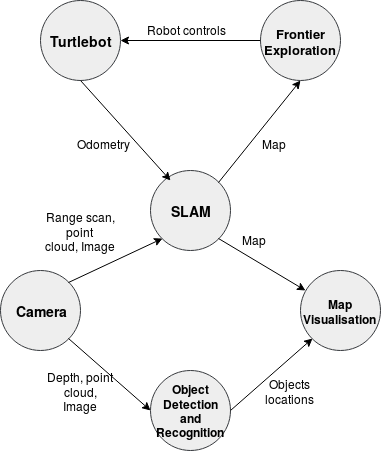
\includegraphics[width=0.5\textwidth]{images/system-diagram.png}
  \label{fig:System Diagram}
\end{figure}

The advantage of using this type of design is it that it maps directly to the way ROS works. A node is equivalent to a ROS node and contains a process while edges are equivalent to ROS topics. This design allows some nodes to be removed, for example frontier exploration and map visualisation and the other nodes will still work as expected. This is useful because the system can developed and tested in modular stages. Similarly nodes can be replaced, for example the Turtlebot and camera can be replaced by a simulation which will provide the same edges meaning their is scope for adaption and code reuse for future projects.

\section{Conclusion}

Formulating requirements provides a clear understanding of the scope of the project. This also allows the system design to be flexible and account for an iterative processes where different modules can be completed and tested in stages. The high-level system is able to capture the requirements and is sufficiently modular. The next chapter will describe the implementation process of the stated design... More***  


%%%%%%%%%%%%%%%%%%%%%%%%%%%%%%%%%%%%%%%%%%%%%%%%%%%%%%%%%%%%%%%%%%%
\chapter{Implementation}
\section{Introduction}

Emphasis the connection between nodes. Tested throughout

\subsection{System Diagram}

\section{Mapping}

I did this because of this which allows this

Integrating with the cameras tricky.

RTABMap has software

More about RVIZ

\section{Frontier Exploration}

why I choose it justify.

How it works brieflfly.

Slowed down
Too fast camera motion for the framerate: If the camera is moved too fast, there will be less features to match between successive frames. RGB images can be also blurry depending of the camera, which decreases the number of good visual matches between frames.
\section{Object Detection and Recognition}
The purpose of the object detection and recognition package is to be able to locate potential objects within a scene, classify them and note their location within the map being built using SLAM.

This package was determined to be written from scratch as it required bespoke functionality however certain other software was consulted such as Find Object \cite{} and Bing\cite{}. Why? Because the detection would primarily be carried out by a mobile robot certain aspects were modelled on lower organisms visual systems. Both of these pieces of research helped form the completed package.

This package was written in Python 2.7 primarily to make use of the ROS and OpenCV bindings which are required. The ROS bindings (Rospy) permits the interfacing of ROS components in Python. It allows nodes to be implemented very quickly at the expense of runtime speed, but this tradeoff was considered acceptable as this project is prototypical and can be ported to the faster C++ API in the future if required. OpenCV is a library of computer vision functions such as displaying, processing and machine learning.


\subsection{Detection}

Similar detection software was consulted and in all cases some form of blob detection was used to determine salient regions, frequently called Regions of Interest (ROI) \cite{HosangBS14}. Blob detection allows areas of a 2D image with similiar parameters such as brightness or colour to be distinguished from their surroundings. Blob detection is a sequential process and each stage is described.  **** What does R-CNN do... hybrid system...

\subsubsection{0. Initial Exploratory Blob Detection}

Initially a naive method was concieved that took SIFT or FAST features as regions of interest within an image and the created a blob around clusters of these features. This method used a handwritten blob creator algorithm that determined blobs based on a closeness value in pixels to the current blob's edge.

 \begin{algorithm}
    \SetKwInOut{Input}{Input}
    \SetKwInOut{Output}{Output}

    \underline{function isNearEdge} $(x,y)$\;
    \Input{External feature vector $x$ and $y$}
    \Output{Boolean}
    Where $blobFeatures$ are current features within the blob\;
    $shortestDistance \leftarrow 10000 $\;
    \For{$vector$ \textbf{in} $blobFeatures$}
    {
    $tempDistance \leftarrow euclideanDistance( x,y,vector ) $\;
    \If {$ tempDistance < shortestDistance $}
    {
    	$shortestDistance \leftarrow tempDistance$
    }
    }
    \lIf {$ shortestDistance < minimumDistance$}
    { 
    	\Return True
    }

    
    \caption{Determine if a given feature is within the distance of a blob.  }
\end{algorithm}

This method generally worked, however it is a very slow and costly function whereby every feature vector has to be compared against every other feature vector but moreover it fundamentally assumed that objects contained more features than their surrounding environments which is flawed. 

The environment that will be encountered when the project is run is unknown but it can be assumed that objects are likely to be found in the environment. The type of environment will be variable but will typically be an office or workplace which will feature some areas of high entropy such as book shelves, exterior windows and patterned carpets. Therefore in some cases the object may have less features than it's surroundings.

\subsubsection{1. Thresholding with Otsu's Method}

Considering this, an assumption was made that potential objects will be in the foreground of an scene. This means that objects can be distinguishable even when there is a high degree of variance in the overall scene. 

To achieve this the grey-scale of the image was thresholded using Otsu's method which creates a histogram of intensity and then chooses an  threshold value to split the image into two classes. This method was chosen because it is very fast and assumes that an image has two kinds of pixel, foreground and background\cite{otsu}. Objects in the foreground are considered to be sparce compared to the background and therefore the class with the lesser number of pixels is determined to be the foreground. In, FIGURE this process correctly distinguishes the high contrast guitar in the foreground. However, the white walls distort this and constitute a great deal of the image (although there are still slightly less white pixels than black here) this could lead to the foreground being incorrectly determined.

\begin{figure}
   \caption{High-Level System Architecture. Consisting of the four main active processes of the project, as well as the passive hardware components (Turtlebot and camera).}
   \centering
   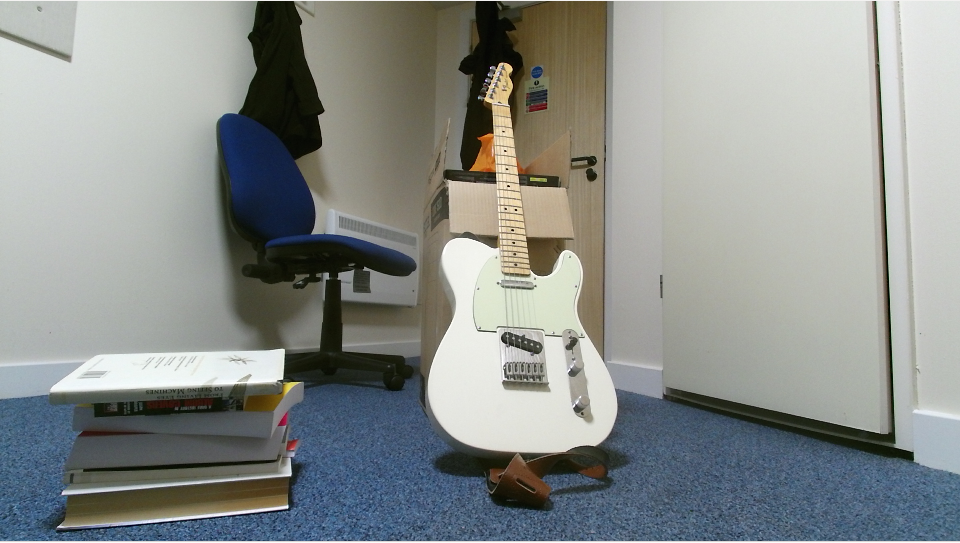
\includegraphics[width=0.475\textwidth]{images/basic.png}
   \hfill
   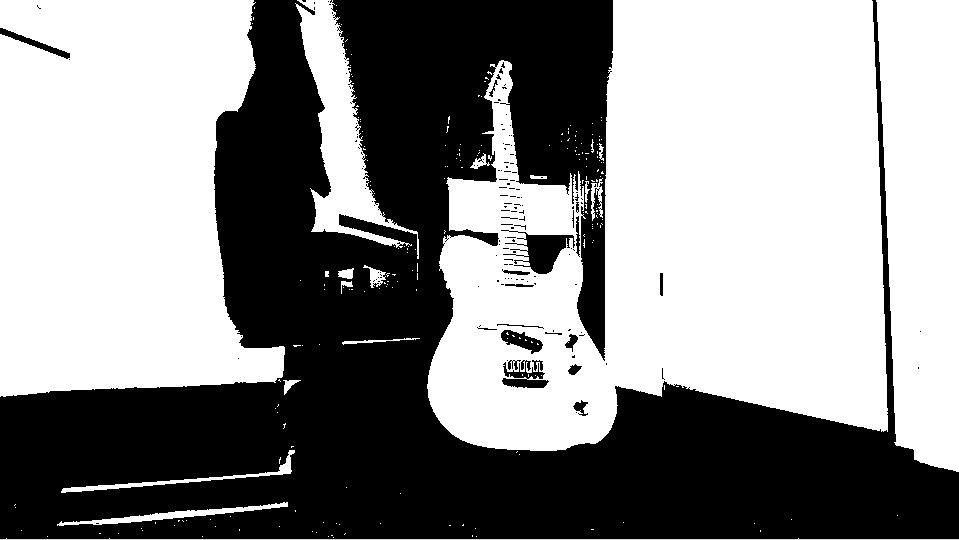
\includegraphics[width=0.475\textwidth]{images/otsu.png}
\end{figure}

\subsubsection{1.5. Calibration Tool}

In some cases large expanses of the same material with the same colour such as carpet or walls can be overrepresented in the mask thus inversing the foreground and the background incorrectly. To mitigate the chance of this happening a calibration tools was written. While running this program the camera can be pointed at a region of the environment that will be subtracted from subsequent image processing. This tool extracts the mean hue, saturation and luminance (HSV) values of the region which is used to subtract other areas which feature a HSV within a certain range of the mean. HSV is used as opposed to RGB or BGR image spaces because it seperates colour from luminance (intesity), this means that changes in lighting such as shadows or sunlight do not affect the detection of similar regions thus produces more accurate masks. SEE APPENDIX


\subsubsection{2. Combining with a Depth Mask}

To properly seperate the foreground the Otsu method is combined with the a depth mask taken from the Kinect or Zed Camera's range finding where a depth threshold is pre-determined. This allows only locations within a certain range to be located therefore considerably improving the the clarity of the foreground. (However it is important to note the books FIGURE are just at the edge of the Kinect sensor's range and not fully rendered.) A morphological operation removeSmallObjects found in the Scikit-Image library is used to perform erosion and dilation based on a specified kernal size, this has the effect of removing small regions of spurious pixels and somewhat provides blobs with well defined edges.

\begin{figure}
   \caption{High-Level System Architecture. Consisting of the four main active processes of the project, as well as the passive hardware components (Turtlebot and camera).}
   \centering
   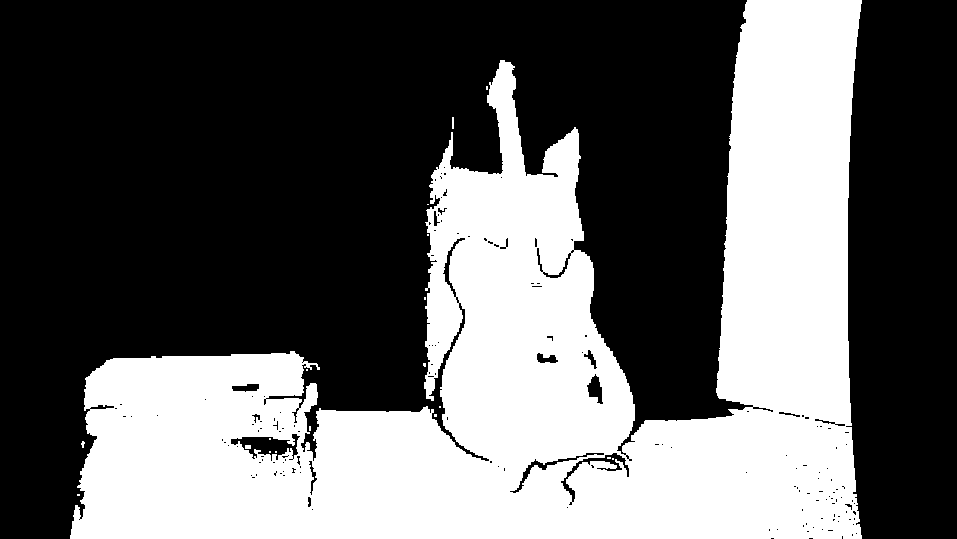
\includegraphics[width=0.475\textwidth]{images/depth.png}
   \hfill
   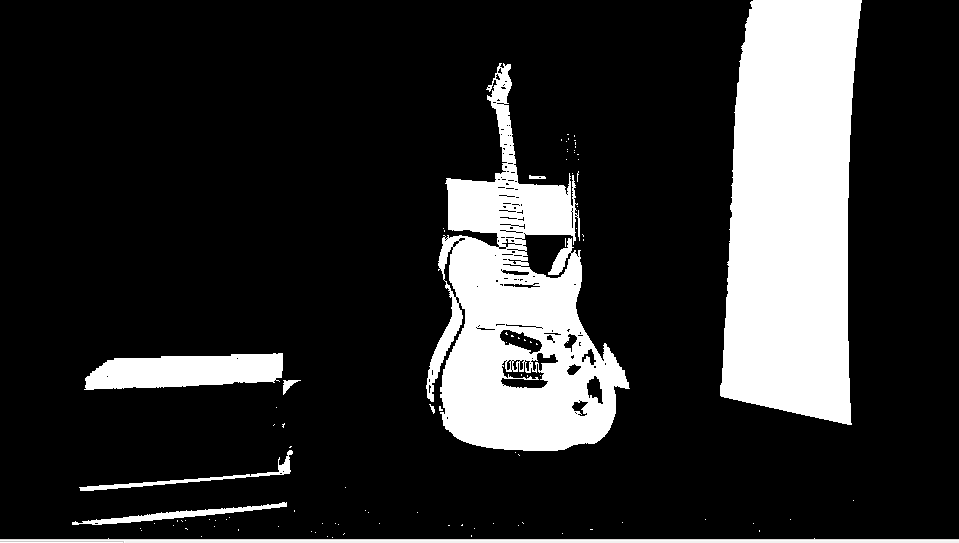
\includegraphics[width=0.475\textwidth]{images/combined.png}
\end{figure}

\subsubsection{3. Clustering}

With the blobs sufficiently seperate from the background they can be clustered with the aim of creating segments. This allows bounding boxes to be defined around each segment forming a region of interest. 

This is similar to how R-CNN finds bounding boxes however in R-CNN the number of clusters is a known variable, usually 2000 and the Selection Search algorithm is used to find this many clusters. In this project the number of potential objects in a scene is unknown and therefore the number of clusters is also unknown, this limits the number of algorithms that can be used.

A clustering algorithm, Density-based spatial clustering of applications with noise (DBSCAN)\cite{} is applicable to this problem as it works with an unknown cluster number and an implementation is provided in in the Scikit-learn package. This has a best case complexity of $O(n log n)$ which is considerably faster the inital clustering algorithm ALGORITHM 1 which has a best case of $O(n^{2})$


DBSCAN has two parameters: $\varepsilon (epsilon)$ which defines the radius around a data point $p$ and a minimum number of points that consist of a cluster $minPoints$

The algorithm can be abstractly described as thus:

    Find $\varepsilon$ neighbours of $p_{n}$ and identify the core points
    
    Find connected components of core points
    
    Assign border points or otherwise outliers
  
Where $N$ is a neighbourhood:
 
Core points are  $N_{\varepsilon} >= minPoints $

Border points are $N_{\varepsilon} < minPoints $ but still reachable from a Core point

Outliers are neither core or border points


Clusters are thus created from the core and border points while outliers in can be discounted.

The algorithm was initially tested with (x,y and the colour image) features however this resulted in a very slow runtime. Offseting this by reducing the step size and desampling the image gave poor overfitted clusters. Therefore (x, y, depth and grey-scale image) was used which produces satisfactory clusters.

 
Using a low $\varepsilon$  value results in many clusters similar to the results found in R-CNN's Selection Search, however, R-CNN classifies every bounding box created from the the cluster. This is not feasible for this project which must be implemented in real-time. Therefore a larger $\varepsilon$ is used which produces larger clusters that fit the blobs closer to their real world images.

\begin{figure}
   \caption{High-Level System Architecture. Consisting of the four main active processes of the project, as well as the passive hardware components (Turtlebot and camera).}
   \centering
   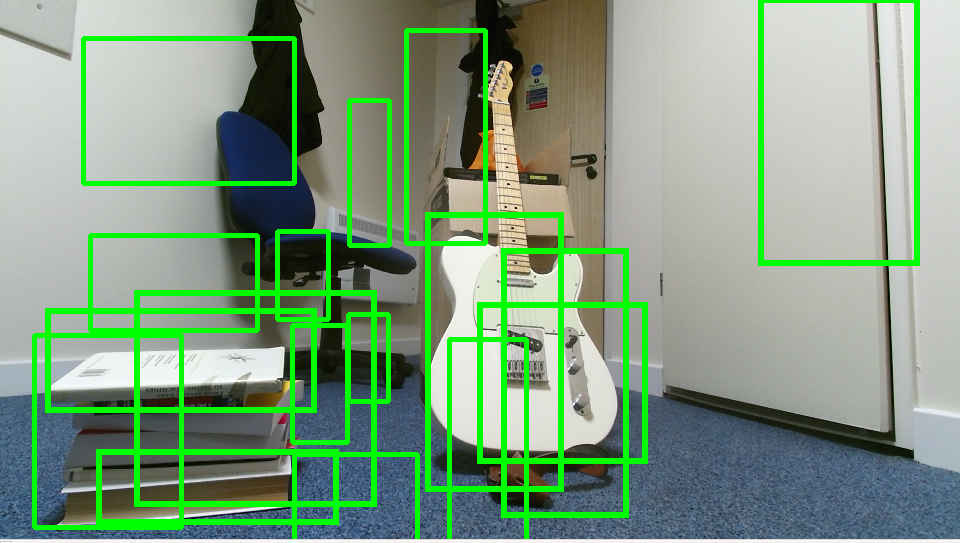
\includegraphics[width=0.475\textwidth]{images/many.png}
   \hfill
   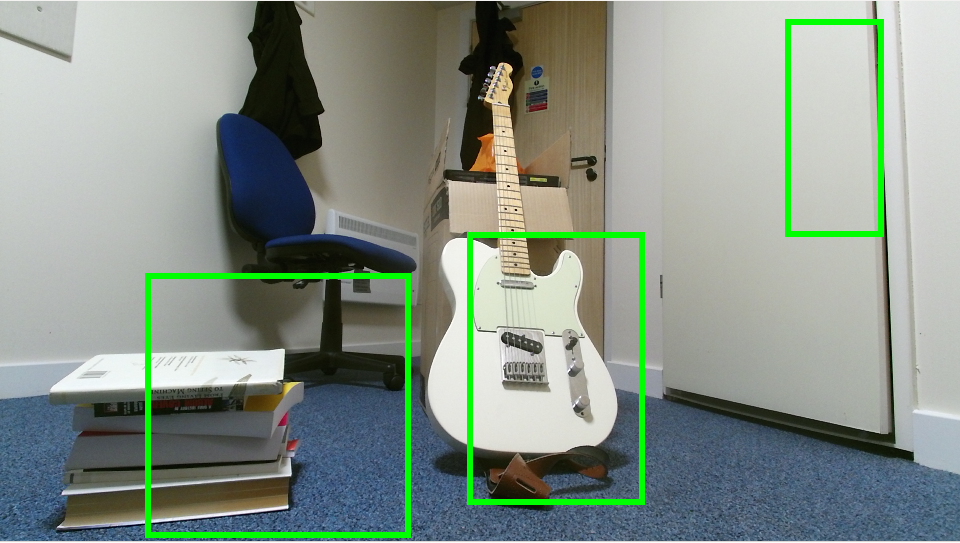
\includegraphics[width=0.475\textwidth]{images/clusters.png}
\end{figure}



\subsubsection{4. Creating Bounding Boxes}

Given the (x, y) points of each cluster a bounding box determined giving a region of interest. This area can then be classified with the assumption that at least part of an object is within the area. Unfortunately, as can be seen in Figure ... some blobs detected are not that interesting notably the area of the door in the right side of the image. This area has very few edges or corners meaning very few noteworthy features. Therefore a minimum threshold of features can be used to determine whether a region of interest is actually interesting thus removing the part of the door. Features will have to be extracted every frame and thus FAST feature detection is used primarily because it is more speed efficient than SIFT.

These objects contained in the bounding boxes exist in a 3D plane meaning that the width and height of each box is arbitary and variable according to the scale and angle of which the object is represented as in 2D. Instead a simplistic of method surrounding the object in a circle is used. The center point of this circle is calculated as the mean point of the previously extracted features for the bounding box, this ensures that the central pixel (u,v) is very likely to be part of the object and not located in the background. The radius of the circle is calculated from the width and height of the bounding box providing a wide location in which the object can be contained.

\begin{figure}
   \caption{FAST features for the stack of books. Note the features are extracted from a RGB image combined with the detected object mask.}
   \centering
   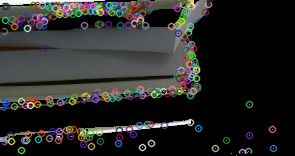
\includegraphics[width=0.5\textwidth]{images/fast.png}
   
\end{figure}

In future iterations of the project the features (possibly using highly discriminate descriptors such as SIFT) of each salient region can be used to create a bag of visual words and be recorded with the label given by the classification process. Over time the histogram of words for each label would increase and become more developed meaning that eventually the system can learn to recognise objects using feature matching. 


\subsection{Classification}

The next step after having detected salient regions within an image is to classify them. Image classification is typically achieved using a CNN which is available in cloud based APIs such as Google Vision, IBM... and also in able to be trained and used locally using Tensorflow. However initially an alternative Haar Feature-based Cascade Classifier was considered before examining a robotic visual memory model was and more successful CNN based classifiers used.

\subsubsection{Haar Cascade}

A Haar Cascade is based on Viola-Jones face detection and has the advantages of being very fast and suitable for real-time applications\cite{viola} as well as having a framework built into OpenCV. The model is trained with positive images of the desired object in different environments at different scales and sizes and with negative images of anything other than the positive image. Creating the positives first required extracting the object so that the background is transparent. This process required different methods for different objects but was tested with a Coca-Cola can. APPENDIX. OpenCV contains a script to take these transparencies and impose them at different perspectives and scales within negative background images which were taken from ImageNet\cite{}. The training stage was also handled by OpenCV and was trained to 10 Adaboost stages. This process took an unbelievably long time and had to be aborted after 9 stages having taken more than 16 hours despite using the maximum amount of memory. The classifier could still be tested after the completed stages and while it did detect the Coca-Cola Can with no occurence of false positives, the training process is too long particularly if a selection of objects need to be detected.    

\subsubsection{Robot Visual Memory Model}

Instead a model was developed inspired by natural visual memory systems, that which allowed a simple hierarchy of objects to be built from exploring an environment. This limited the need to recognise a large amount of objects while also recognising that not all regions of interest are actually important objects within the room. Frogs neural responses are triggered by goal based features where features are remembered more readily if they constitute part of or all of a goal. For example the goal of feeding is associated with black ellipsical objects indicating flies, while being carnivorous a seed pod shaped object would less likely be remembered.

This model is invoked after a salient object has been detected. Once an object is classified it is determined to either exist in the robot's long term or short term memory. The long term memory constitute of objects which have been defined. These are objects which are necessary for a goal, where the first step of achieving this goal is correctly identifing these objects. This means the objects are distinct and important such as a computer, coffee maker or in the case of Figure, a guitar. When the Turtlebot explores a room the first question asked when a region of interest has been detected is "Is this one of the goal-based objects?" If the result is affirmative then the object is remembered within it's environment perpetually in long term memory. 

On the otherhand if the object is not pre-defined it is stored in short term memory where it will be forgotten after time. When a mapping and exploration session is finished and all objects have been classified, objects which currently exist in STM are forgotton while objects in LTM are associated and assumed to exist with the completed map.

Because the project intends to map whole rooms, the manner in which STM is dumped after completion is comparable to the concept of event boundaries or the "Doorway effect". \cite{} This phenomena occurs when human's leave rooms they have a tendancy to forget what they were previously doing. This exists because spatial changes such as entering a bathroom often correspond with physical and mental changes such as needing to use the bathroom and thus can readjusting our hierarchy of memories.

\subsubsection{Implementing the Memory Model}

Two different kinds of CNN classifiers are used to determine if an object will be stored in LTM or STM. 

The first is the TensorFlow MobileNet CNN which is trained with a selection of objects that if found will be stored in LTM. MobileNet was chosen over other types of image classifiers because it can operate in real-time with performance testing indicating that it takes between 0.1 and 0.3 seconds to classify from six potential objects. Using it through TensorFlow simplified the training process which only took roughly 30 minutes. The training sets were chosen by bulk from Google Images. This allowed regions of interest to be scored from the defined objects, if the score was less than a confidence level (such as 0.9) then the object is considered to be important and is not stored in LTM.

The second classifier is the Google Vision API. A cloud based classifier was chosen over training one from scratch as training one to contain all the types of objects in office based environments would take too long. Similarly using a pre-trained classifier locally such as Inception \cite{} would potentially schew the classifications with irrelevant labels such as animals or landscapes. An image is send to the API and the response contains the most confident single label and score of the object. This compares to the IBM classifier which returns all labels with all the scores resulting in situations where an object can be labeled a car and a tomato and both have a score of 0.9 which is not as useful for the purposes of this project. 

Illustration of the scoring

Another advantage of the Google Vision API was discovered through sustained use in that the labels it provides are very vague. For example a chair is labeled as furniture and bottles are labelled as products. As this classifier is determining short term memories it is enough for the robot to know what an area of an environment vaguely is as it is not concerned with the goal of finding important objects. Unfortunately the Google Vision API is slow, with classifications taking from 0.3 to 1 second depending on internet connectivity and speed. However, a buffer of request is formed while also noting the location where the object is found meaning the robot can operate in real-time and correctly classify objects at locations in the map being built.



\subsubsection{Adding markers}



These two classifiers are combined in a process where on discovering a new region of interest...

Objects need to be detected in 3D and previously classified objects need to persist meaning that the same object is identified between frames.


This is achieved through the use of ROS markerArray. A marker is an (x, y, z) point which exists in a coordinate frame in this case the map frame. There are too cases that need to be accounted for: 1) A new object is detected and 2) An existing object is detected.


If a new object is detected and classified an approximate location of this object is calculated by finding the mean feature point of the object and finding the corresponding value from the point cloud image. This is transformed into an (x, y, z) point in the map coordinate frame and is published as a marker with an associated label in ROS. 

For every 2D region of interest found a test is made to see if a real-world marker exists within it's vincinity. This is calculated by assuming an object has a sector where it is highly likely this object is the sole occupant. This avoids seperate markers from being created for what is the same object. Considering a point $P (x, y, z)$  and a sphere with a centre $ C (x_{0}, y_{0}, z_{0}) $ and radius $r$ . $P$ exists within $C$ if $(x-x_{0})^{2} +  (z-z_{0})^{2} + (z-z_{0})^{2} <r^2$

The complete algorithm for the process of classification can be can be seen in Figure... This process provides a way remember locations of discovered objects in a map and to minimize costly classifications to only when new objects are discovered. 

ALGORITHM

These markers are displayed in RVIZ as text at the relevant point in the map. A simple GUI in OpenCV was created which also displayed the detected objects.
Red = long term, Yellow = STM

\subsection{Conclusion}


%%%%%%%%%%%%%%%%%%%%%%%%%%%%%%%%%%%%%%%%%%%%%%%%%%%%%%%%%%%%%%%%%%%
\chapter{Evaluation}

A testing stategy was developed which would allow the project to be tested in its entirity this involved a set of three expriments to ensure the project was successful or highlight areas for improvement.

\section{Testing}
\subsection{Experiments}

Three experiments were developed to determine whether the project objective has been achieved and to what extend, due to the fact that specific hardware was required and ongoing issues with the Turtlebot the experiments were completed in one sitting at the end of the project development period. 

The project objective: 

The Turtlebot will autonomously create a 3D map of an unknown room while creating an inventory of classified and localised objects in the map.

Five qualitive measures are used determine if parts of an experiment were successful, a more quantitive assessment would require more advanced software to compare completed maps and pointclouds with precise ones and is out of the scope of the project. 

- Adequate Performance - The map is produced with no noticable delay in the robot's movements 

- Accuracy of a map - The map produced is complete and the shape of the room is easily distinguishable

- Accuracy of point cloud - The point cloud does not feature any repition or gaps and objects are distinguishable.

- Successfulness of classification - The guitar is identified once.

- Successfulness of object detection - Some objects are detected and classified with vaguely relavent labels.

\subsubsection{Experiment Setup}

A small-medium enclosed room was chosen to perform testing. This allows the room to be mapped in a reasonable time due to issues pertaining to the Turtlebot battery life and temperamental connectivity between the laptop and the Kobuki and is free from human disturbances. The room was adequately lit with no natural light. 

A guitar is placed in the room, this has been chosen as the goal of the robot with the MobileNet having been trained to detect guitars. It is the only significant object in the room with the rest consisting of a chair, bag, bin, wardrobe, bed and desk.

An Xbox Kinect v2 was used as the Turtlebot camera sensor and was connected the Lenovo Ideapad Y700 which had the RTABMap Visualisation tool and RViz open.


DIAGRAM
Map of the room accurate

FIGURE words
A map features light gray for discovered with no barriers, black barriers, medium grey for undiscovered.

Yellow = STM
RED = LTM


\subsubsection{Experiment 1}

Does the system autonomous map the environment?

Hypothesis: The Turtlebot will successfully explore the two sections of the room, the map produced will be relatively accurate but may miss areas out in the narrower part of the room.

Result A: 

- Adequate Performance - n/a

- Accuracy of a map - Poor

- Accuracy of point cloud - Poor

- Successfulness of classification - n/a

- Successfulness of object detection - n/a

Process: 
The Turtlebot was placed 60-70 cm from the wall Figure A. The Turtlebot span less than 90 degrees and RTABMap indicated that odometry had been lost and mapping would not continue. The process was terminated.

Remarks: The Turtlebot was so close to the wall that the field of vision for the Kinect was entirely consumed by a white wall and no features and thus no landmarks could be extracted for SLAM to work. This indicates that the start position of the robot is very important.Unfortunately, nothing can be done to mitigate the program and thus the user must decide the start position.


 \begin{figure}
   \caption{RTABMap visualisation indicating that no landmarks can be found and odometry has been lost.}
   \centering
   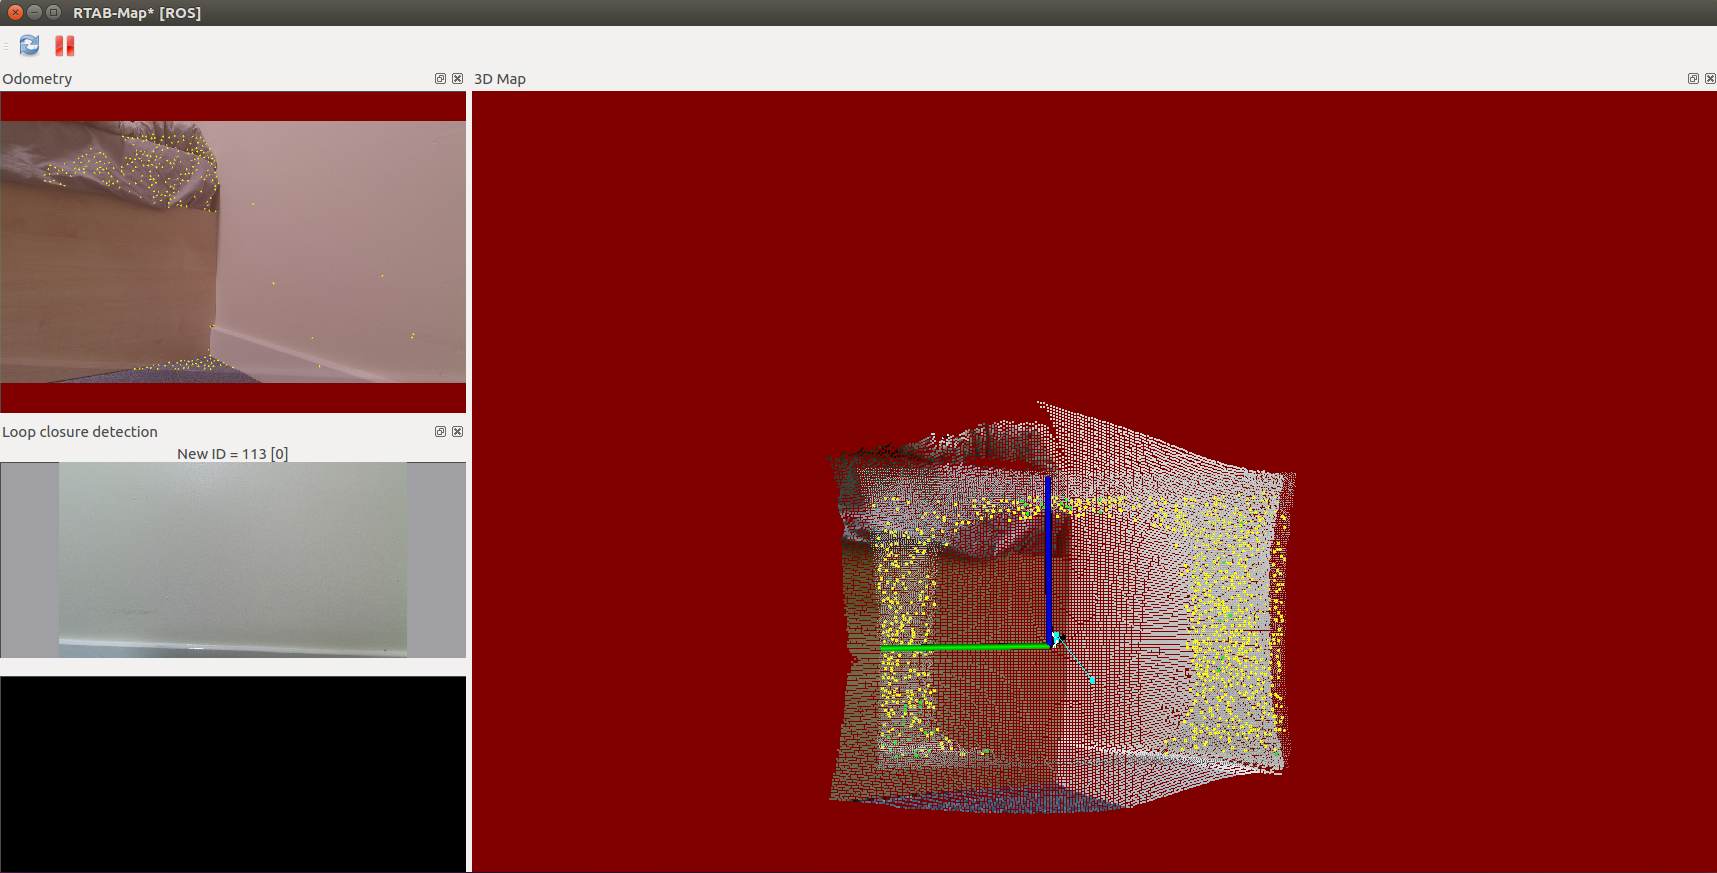
\includegraphics[width=0.475\textwidth]{images/resulta.png}
   \hfill
   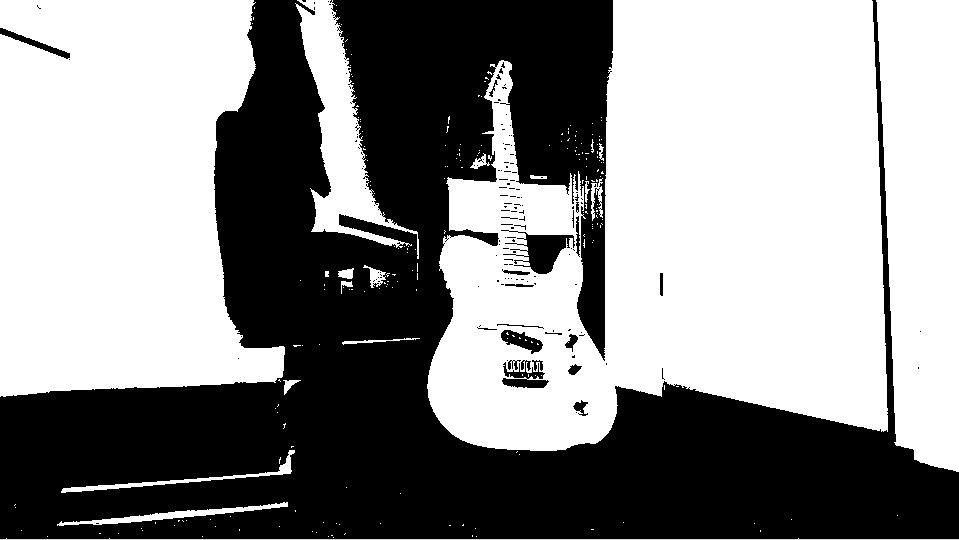
\includegraphics[width=0.475\textwidth]{images/otsu.png}
\end{figure}

Result B: 

- Adequate Performance - \checkmark

- Accuracy of a map - Acceptable

- Accuracy of point cloud - Good

- Successfulness of classification - n/a

- Successfulness of object detection - n/a


Process: The Turtlebot was placed in the center of the room equidistant from walls. The Turtlebot proceeded to begin explore and map the large section of the room. The narrow part of the room was visited but was not traversed the whole length. The process terminated naturally.

Comments: The Turtlebot produced an accurate point cloud of the image. The  map is generally accurate but with some walls slightly distorted and a shadowy region underneath a desk producing a cluster of thick barriers in this area (Black region at bottom of map).The map is missing the circumference where the Turtlebot began as the Kinect range scanner has a minimum threshold. The frontier exploration algorithm relized leased this area was still enclosed so did not explore it. However, this could be completely solved by editing the frontier exploration source code to account for non-discovered regions within an enclosed area. 
\begin{figure}
   \caption{Red arrow indicating the start pose}
   \centering
   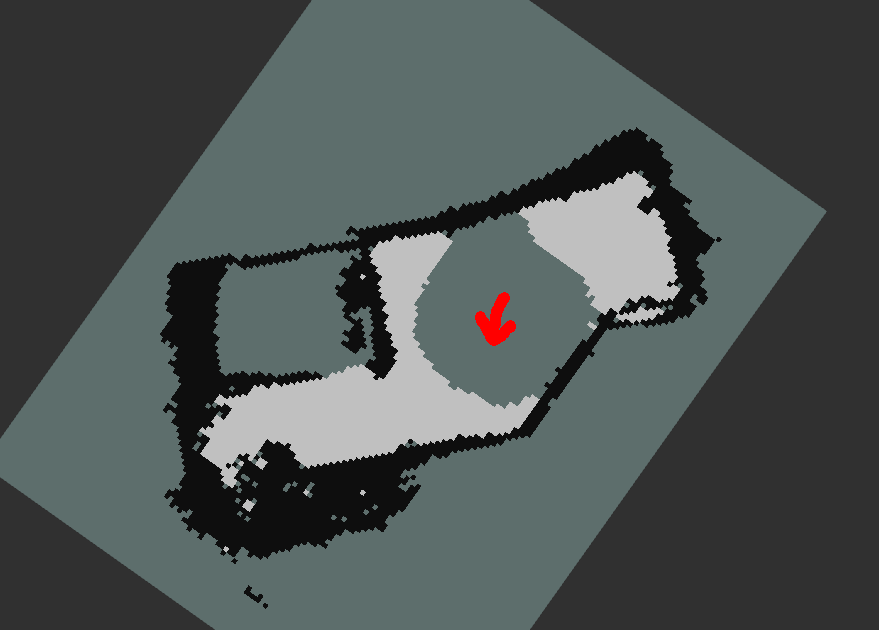
\includegraphics[width=0.475\textwidth]{images/exp1map.png}
   \hfill
   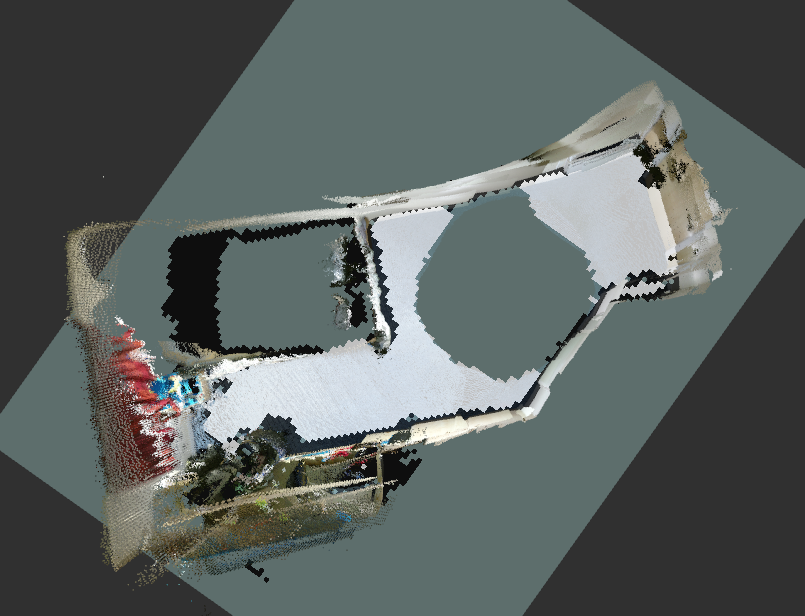
\includegraphics[width=0.475\textwidth]{images/ex1pc.png}
\end{figure}


\subsubsection{Experiment 2}

Can objects be detected while mapping with manual teleoperation?

Hypothesis: The Turtlebot will successfully map the room including the start position. The guitar will successfully be detected and classified. Other objects will be detected in the room and classification should be somewhat accurate.



Results: 

- Adequate Performance - \checkmark

- Accuracy of a map - Good

- Accuracy of point cloud - Good

- Successfulness of classification - Good

- Successfulness of object detection - Acceptable

Process: The Turtlebot was controlled using teleoperation to all areas of the room. The guitar was approached intially head on and then from the sides and was classified successfully and only once. Other regions of the room were classified.

Comments: Using teleoperation resulted in a map with more coverage than Experiment 1. However, due to non fluid angles that the Turtlebot was moving in there are some incorrect doubled barriers. The guitar is successfully located and classified. Other objects are detected but while most of these are correctly identified such as wall, others are given very vague descriptors such as blue. (Presumeably because the furniture is a blue colour). This may be because the bounding box used to enclose the object was too restrictive  thus and it can only be identified as a whole


 \begin{figure}
   \caption{Red arrow indicating the start pose}
   \centering
   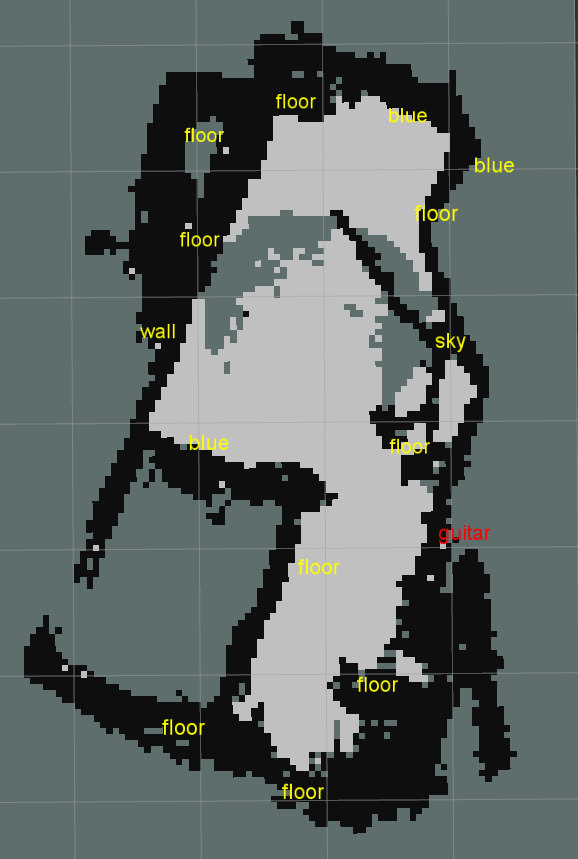
\includegraphics[width=0.5\textwidth]{images/ex2.png}
\end{figure}

\subsubsection{Experiment 3}

Can objects be detected while autonomously mapping in real-time?

Hypothesis: The Turtlebot will successfully map the room but not the starting location. The guitar will successfully be detected and classified. Other objects will be detected in the room and classification should be somewhat accurate.

Results: 

- Adequate Performance - \checkmark

- Accuracy of a map - Good

- Accuracy of point cloud - Good

- Successfulness of classification - Good

- Successfulness of object detection - Good 

Process: The Turtlebot was placed in the center of the room equidistant from walls. The Turtlebot proceeded to begin explore and map the large section of the room. The guitar was classified successfully and only once. Other regions of the room were classified. 

Comments: The map suffers the same missing regions as in Experiment 1. However the point cloud is complete. The guitar is successfully located and classified. Interestingly the STM classifications are better than in Experiment 2, giving the furniture descriptor for the wardrobe and the chair. A floor was detected outside of the map.

Experiment 3 was successful it produced the most accurate map and point cloud despite missing the starting location. The guitar was located and classified correctly as well many other objects in the room such as the wardrobe and chair being given a furniture descriptor. This may be because the frontier exploration package used is very conservative with movements which means objects can be detected from a distance making them distinguishable from their background. The floor was detected outside of the map which may have been caused by the pointcloud readjusted itself during the mapping process leaving the marker at it's original location.

 \begin{figure}
   \caption{Red arrow indicating the start pose}
   \centering
   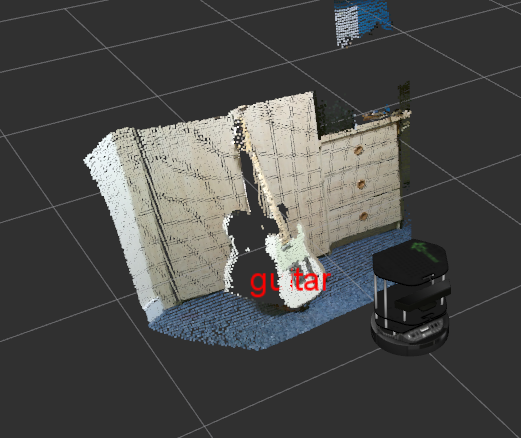
\includegraphics[width=0.475\textwidth]{images/ex3.png}
   \hfill
\end{figure}

 \begin{figure}
   \caption{Text partially obscured by point cloud}
   \centering
   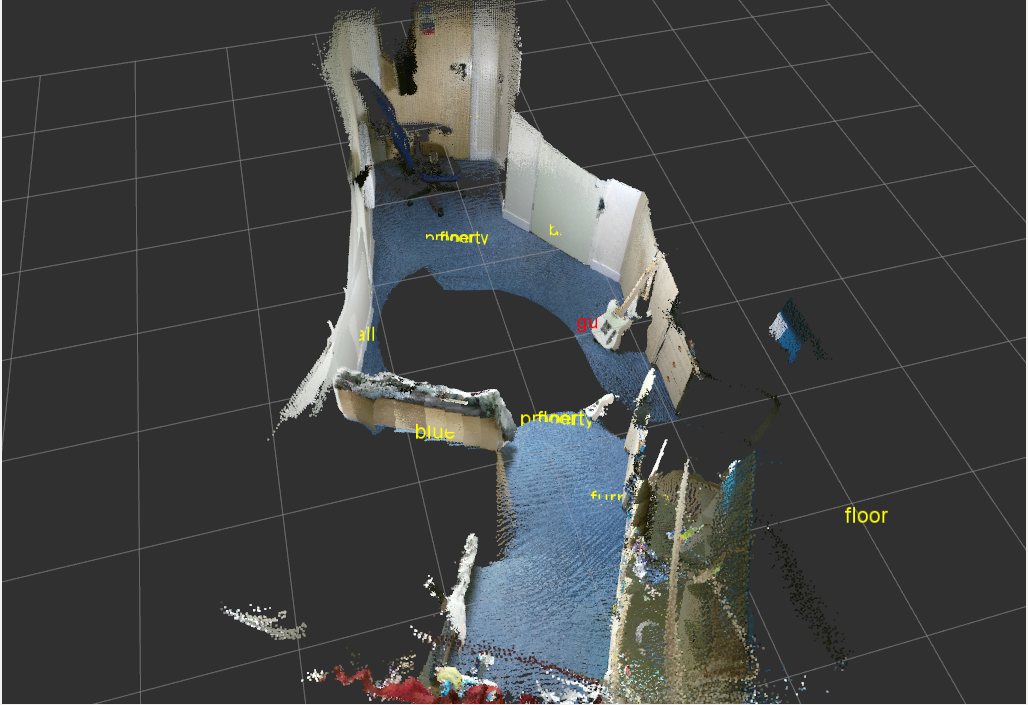
\includegraphics[width=0.8\textwidth]{images/ex3pc.png}
   \hfill
\end{figure}

\section{Conclusion}

The hypothesises stated are all proved correct and thus the project objectives have been achieved, with an environment accurately mapped autonomously and the contents classified successfully. The requirements indicated for completion in the first version were all completed. Results varied across experiments and with even slight changes to the setup giving very different readings. While the individual components were tested iteratively during the implementation stage it was difficult and time consuming to do comprehensive tests of the whole project until all components were completed. The overall project could be improved by implementing solutions to some of the problems found during the testing process. This would essentially constitute a  second version whereby other requirements could be completed also. 

%%%%%%%%%%%%%%%%%%%%%%%%%%%%%%%%%%%%%%%%%%%%%%%%%%%%%%%%%%%%%%%%%%%
\chapter{Conclusion}\label{conclusion}
\subsection{Future work}

incorporate active detection of features next time.

A signature map can be created from the locations of objects in the map. Indicating whether a floor is here. Similar to geological mapping

Create database of objects


\appendix % first appendix
%%%%%%%%%%%%%%%%%%%%%%%%%%%%%%%%%%%%%%%%%%%%%%%%%%%%%%%%%%%%%%%%%%%
\chapter{First appendix}

\section{Section of first appendix}

%%%%%%%%%%%%%%%%%%%%%%%%%%%%%%%%%%%%%%%%%%%%%%%%%%%%%%%%%%%%%%%%%%%
\chapter{Second appendix}

%%%%%%%%%%%%%%%%%%%%%%%%%%%%%%%%%%%%%%%%%%%%%%%%%%%%%%%%%%%%%%%%%%%
% it is fine to change the bibliography style if you want
\bibliographystyle{plain}
\bibliography{mproj}
\end{document}
